\documentclass{beamer}
\usepackage{dsfont}
\usetheme{CambridgeUS}
\mode<presentation>
\title[Exploring R]{Exploring R via Fourier Series}
\institute[NIC]{Near Infinity Corporation}
\author[Ed MacDonald]{Ed MacDonald \\ \texttt{emacdona@nearinfinity.com}}
\renewcommand\mathfamilydefault{\rmdefault}
\usepackage{verbatim}
\definecolor{demph-color}{gray}{0.80}
\begin{document}

\begin{frame}
   \titlepage
\end{frame}

\begin{frame}
   \frametitle{Fourier Series}
   \[
      \color<2->{demph-color}{x(t) = }
         \alert<2>{a_{0}}
         \color<2->{demph-color}{+ \sum_{n=1}^{\infty}}
         \alert<2>{a_{n}} 
         \color<2->{demph-color}{\cos n} 
         \alert<2>{\omega_{0}} 
         \color<2->{demph-color}{t + }
         \alert<2>{b_{n}} 
         \color<2->{demph-color}{\sin n} 
         \alert<2>{\omega_{0}} 
         \color<2->{demph-color}{t}
   \]
   \color<2->{demph-color}{where:}
   \begin{align}
      \alert<2>{\omega_{0}} 
      &\color<2->{demph-color}{= 2 \pi f_{0} = \frac{2\pi}{T_{0}}} \notag \\
      \alert<2>{a_{0}} 
      &\color<2->{demph-color}{= \frac{1}{T_{0}} \int_{T_{0}} x(t) \, dt} \notag \\
      \alert<2>{a_{n}} 
      &\color<2->{demph-color}{= \frac{2}{T_{0}} \int_{T_{0}} x(t) \cos n\omega_{0}t \, dt} \notag \\
      \alert<2>{b_{n}} 
      &\color<2->{demph-color}{= \frac{2}{T_{0}} \int_{T_{0}} x(t) \sin n\omega_{0}t \, dt} \notag  
   \end{align}
\end{frame}

\begin{frame}
   \begin{figure}
   \includegraphics[scale=0.40]{squareWave10.pdf}
   \end{figure}
\end{frame}

\begin{frame}
   \begin{figure}
   \includegraphics[scale=0.40]{squareWave50.pdf}
   \end{figure}
\end{frame}

\begin{frame}
   \begin{figure}
   \includegraphics[scale=0.40]{triangleWave3.pdf}
   \end{figure}
\end{frame}

\begin{frame}
   \begin{figure}
   \includegraphics[scale=0.40]{triangleWave20.pdf}
   \end{figure}
\end{frame}

\begin{comment}
\begin{frame}
   \frametitle{What is true of these two pictures??}
   \begin{columns}
      \begin{column}{5cm}
         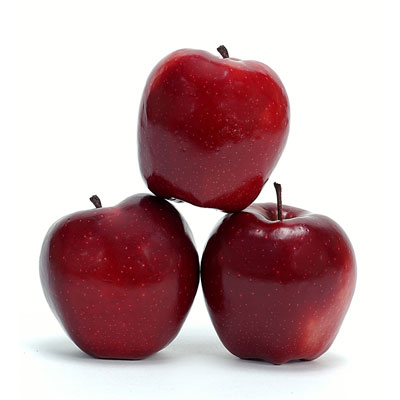
\includegraphics[width=4cm,height=4cm]{images/apples.jpg}
      \end{column}
      \begin{column}{5cm}
         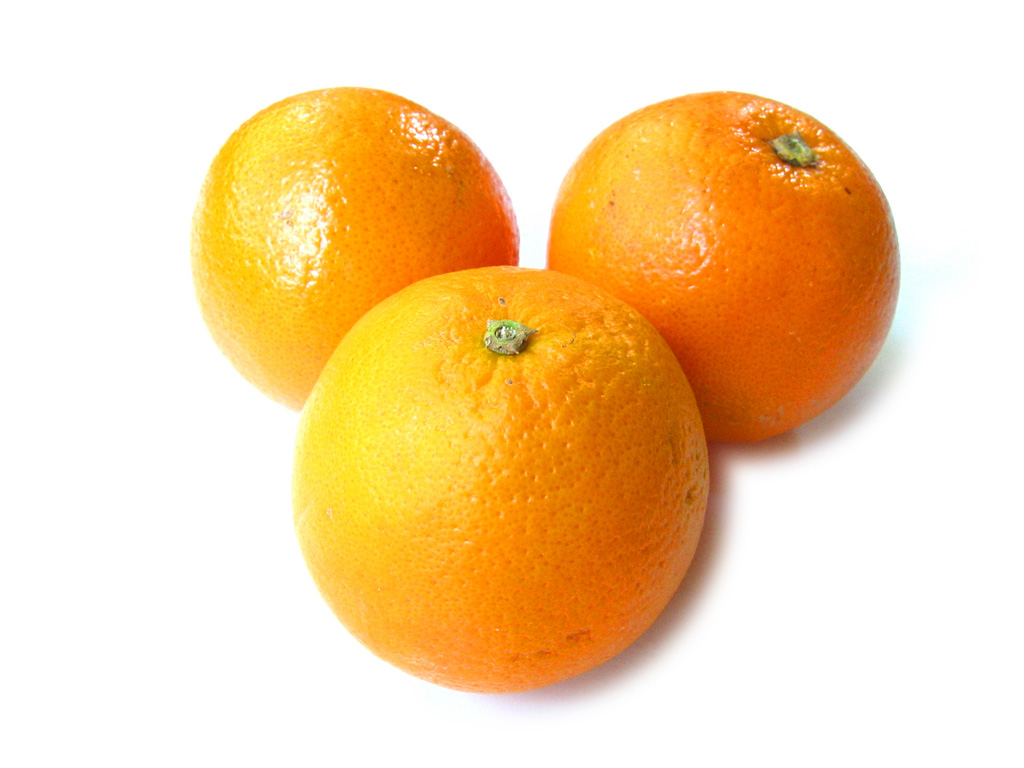
\includegraphics[width=4cm,height=3cm]{images/oranges.jpg}
      \end{column}
   \end{columns}
\end{frame}

\begin{frame}
   \frametitle{What is a Natural Number?}
   1858: Giuseppe Peano born\\
\end{frame}

\begin{frame}
\end{frame}
\end{comment}

\end{document}

